\subsection{Can Photovoltaic Systems Be Used Effectively for this Application?}

\paragraph{}
Photovoltaic systems are being considered for this project due to their nature to produce electricity in DC form naturally. By doing so this negates the need for converting the power from DC to AC or vice versa. As discussed, this reduces inefficiencies and allows for the opportunity to produce an overall increased efficiency system compared to those traditionally used in commercial buildings today. 

\paragraph{}
To quantify the benefits of PV systems when considering the application of Extra Low Voltage DC power Distribution.

\begin{itemize}[noitemsep,nolistsep]
\item Photovoltaic panel options
\item Brisbane solar production curve analysis
\item Approximate losses of Photovoltatic system
\end{itemize}

%%%%%%%%%%%%%%%
%							PV PANELS
%%%%%%%%%%%%%%%
\subsubsection{PV Panel Overview} \label{section:PV-panels}

\paragraph{}
There are two main types of Photovoltaic cells; monocrystalline and polycrystalline \cite{Haberlin2012}. They are both based on crystalline silicon. Crystalline silicon is silicon that has solidified into atoms that are arranged in a crystal lattice \cite{Haberlin2012}. From this definition, it is intuitive from their names that monocrystalline is when the silicon has solidified into a large single crystal and polycrystalline is many crystals in various orientations. Production of a monocrystalline crystal is energy intensive and pulling a complete single crystal is time consuming \cite{Haberlin2012}.      

\paragraph{}
The efficiency of to two main variations of solar panel are fairly equivalent in efficiency in modern times. Overall when comparing costs and efficiencies, it is generally the best option to choose a monocrystalline panel \cite{Haberlin2012}.The additional factors to consider are mounting systems, control system incorporation, direction of tilt and azimuth \cite{Haberlin2012}.  

%%%%%%%%%%%%%%%
%							BRISBANE SOLAR
%%%%%%%%%%%%%%%

\subsubsection{Brisbane Solar Data}

\paragraph{}
As Brisbane, Queensland, Australia is the test location for this thesis the solar curve must be understood. These graphs can also be known as solar potential and outline the times of day in an area. This is an important factor when considering where and how to mount photovoltaic panels for optimal production efficiency. This graph will change throughout the year as seasons change the the timing of the sunrise and sunset alters. 

\paragraph{}
To produce an accurate estimate of solar production in Brisbane, System Model Advisor (SAM) was used. SAM is a free piece of software for simulating photovoltaic systems. The model was established with Brisbane as a location and it automatically importants and caluclates with appropriate data. This is shown in Figure \ref{fig:SAM-test1-weather}. 

\begin{figure}[H]
	\hfill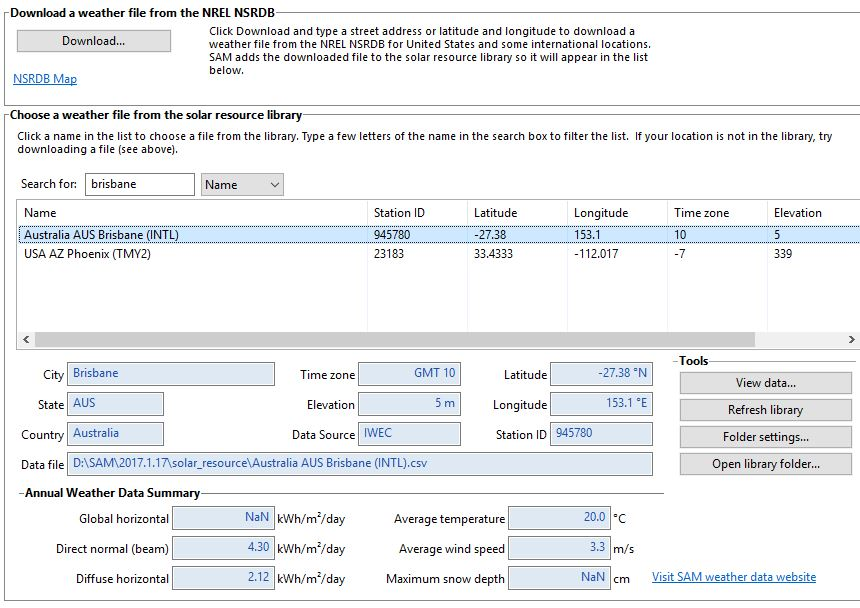
\includegraphics[width = 120mm]{images/sam/test1-weather}\hspace*{\fill}
	\caption{SAM System Design: Weather Settings} 
	\label{fig:SAM-test1-weather}
\end{figure}

\paragraph{}
For module testing, a Suntech Power STP250-20/Wd was chosen for two reasons. These reasons are firstly, that the QUT Project in P Block uses these same modules so the comparison of sites will be more accurate and provide a more detailed analysis. Secondly, 250\,W panels are an average size in the industry as well as monocrystalline being considered the best overall option as discussed \cite{Haberlin2012}. Similarly, the Power-One PVI-3.6-OUTD-US because these are used throughout QUT. In events where 3.6\,kW\,AC or 3.7\,kW\,DC is insufficient, the larger model Power-One PVI-10-OUTD-US will be used for modelling. This test was purely for weather data so the system design is fairly insignificant.  

\paragraph{}
As discussed, during the year the solar curve will change as Figure \ref{fig:SAM-test1-monthlyirradiance} below. To provide a more detailed look, SAM exported hourly data for irradiance over an entire year which was averaged out to display a yearly average irradiance curve in Figure \ref{fig:SAM-test1-dailyirradiance}. These two images outline how Brisbane is a strong contender for installations of photovoltatic systems due to high irradiance levels for the majority of the year.  

\begin{figure}[H]
	\hfill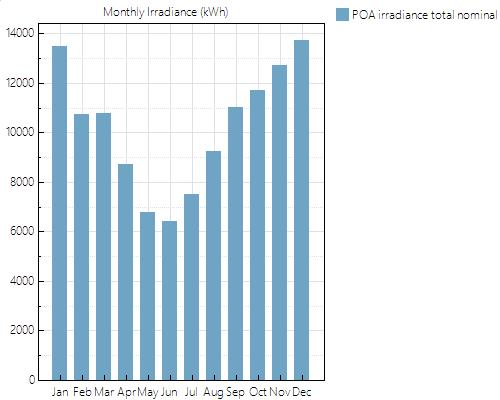
\includegraphics[width = 120mm]{images/sam/test1-monthlyirradiance}\hspace*{\fill}
	\caption{SAM System Design: Brisbane Monthly Irradiance} 
	\label{fig:SAM-test1-monthlyirradiance}
\end{figure}

\begin{figure}[H]
	\hfill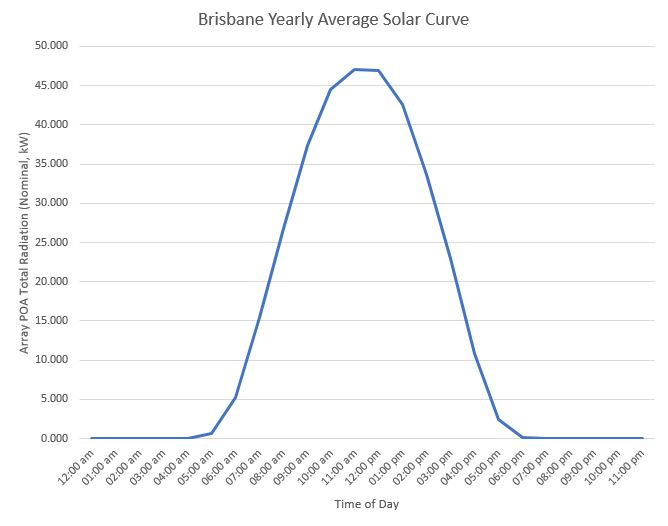
\includegraphics[width = 120mm]{images/sam/test1-dailyirradiance}\hspace*{\fill}
	\caption{SAM System Design: Brisbane Monthly Irradiance} 
	\label{fig:SAM-test1-dailyirradiance}
\end{figure}

%%%%%%%%%%%%%%%
%							LOSSES
%%%%%%%%%%%%%%%
\subsubsection{Losses}

\paragraph{}
Within a power system there are multiple stages of losses. To approximate these losses for a traditional AC Photo-Voltaic system with inverters included, a non-commercially free software package called System Model Advisor (SAM) is available. This program allows the user to input the chosen panels, inverters, tilt angle, shading factors and the azimuth. 

\paragraph{}
To model the test system, a standard module of 250\,W\,Peak was chosen from the SAM module selector. Specifically, a SunPower SPR-250NX-BLK-D with a maximum power production of 249.952\,W and nominal efficiency of 20.09\,\% was selected. This module is intended to represent an average system to give a reasonable quantity to losses to expect for future analysis. 

\paragraph{}
For this level of analysis, again an average inverter requires select to calculate the approximate losses expected from an AC PV system. Because this installation is expected to be incorporated into a commercial building, a 20\,kW inverter was selected. A standard inverter was chosen over micro-inverters due to the increased efficiency they generally provide in larger than residential installations \cite{MicroInverterThesis}. The specific model selected is the SMA America:SB3800TL-US-22 with a 96.2\,\% weighted efficiency and of course a 240\,V\,AC nominal AC output for feeding into existing power infrastructure. 

\paragraph{}
For the test model, strings were made of 30 panels with 8 strings in parallel to simulate a 60\,kWp system. There are a variety of assumptions that were made in order to model and approximate losses including those listed below. These losses are represented in Figure\ref{fig:SAM-Model-1}. 

\begin{itemize}[noitemsep,nolistsep]
	\item Location of Brisbane, Australia with automatically imported weather data
	\item Tilt of 5 degrees
	\item Azimuth of 0 degrees (North facing)
	\item Ground Coverage Ratio (GCR) of 0.1 therefore assuming minimal shading
	\item Flat mounted onto roof
\end{itemize}

\begin{figure}[H]
\hfill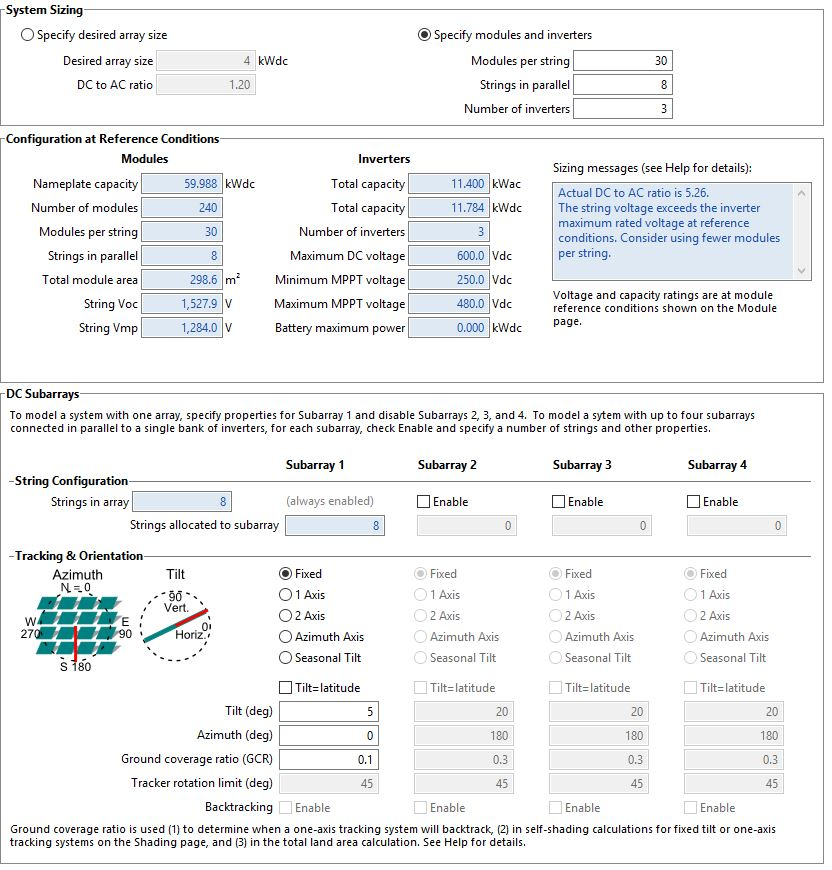
\includegraphics[width = 120mm]{images/sam-1-system-design}\hspace*{\fill}
\caption{SAM System Design: Test Model 1} 
\label{fig:SAM-Model-1}
\end{figure}      

\paragraph{}
SAM results indicate the losses approximated over one year of data and simulations. As can be seen from Figure \ref{fig:SAM-Model-2}, the major losses are from soiling, the module, inverter clipping and DC wiring. Of those, the proposed DC system could remove the 54.134\% loss from the inverters and incorporate a more efficient DC to DC converter.   

\begin{figure}[H]
\hfill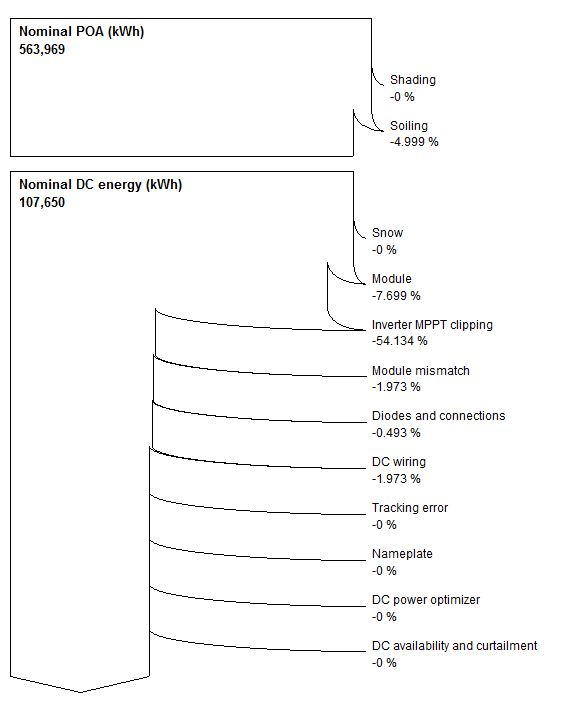
\includegraphics[width = 120mm]{images/sam-1-system-losses}\hspace*{\fill}
\caption{SAM System Design: Test Model 1 Losses} 
\label{fig:SAM-Model-2}
\end{figure}

%%%%%%%%%%%%%%%
%							CONVERTERS
%%%%%%%%%%%%%%%

\subsubsection{Converters}

\paragraph{}
To successfully install the proposed system by adding DC electricity into a power distribution system, the voltage and current produced will require regulation. In existing AC installations, the inverter that converts from produced DC to appropriate AC operates as a regulator and voltage level control system. Because that device is no longer a consideration, there are additional efficiency benefits. Unfortunately an alternative device is required that will add partial inefficiencies. The STP250-20/Wd used for analysis has a production curve represented by below in Figure \ref{fig:PV-Module-Spec-Graph} \cite{website:SuntechModule}.

\paragraph{}
Figure \ref{fig:PV-Module-Spec-Graph} displays the curve representing voltage, current and power.

\begin{figure}[H]
	\hfill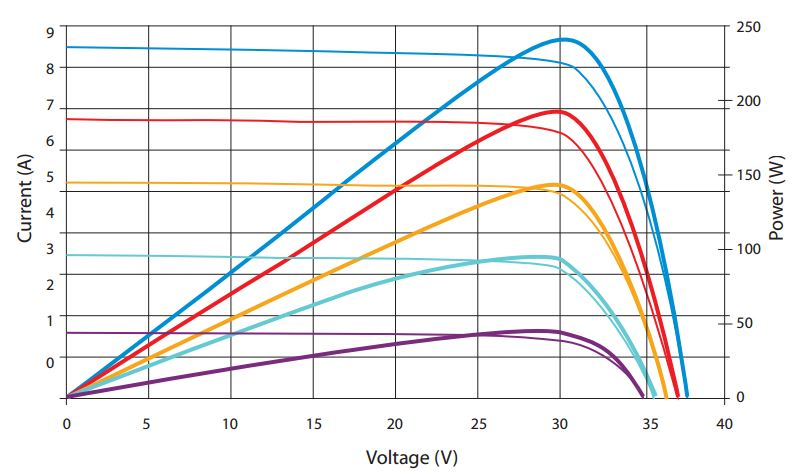
\includegraphics[width = 120mm]{images/sam/pv-module-current-voltage-graph}\hspace*{\fill}
	\caption{SAM System Design: PV Module Current Voltage Power Graph \cite{website:SuntechModule}} 
	\label{fig:PV-Module-Spec-Graph}
\end{figure}

%%%%%%%%%%%%%%%
%							MOUNTING
%%%%%%%%%%%%%%%

\subsubsection{Mounting of Modules}

\paragraph{}


%%%%%%%%%%%%%%%
%							ANSWERING THE QUESTION
%%%%%%%%%%%%%%%

\subsubsection{Suitability}

\paragraph{}
The general question for this section is whether or not photovoltatics could be employed to power an extra low voltage DC power distribution system for a commercial building. Summarising the information discussed above, it is certainly feasible that this is possible due to photovoltatic's ability able to produce DC electricity naturally and the losses being reduced. A test model must be produced and a comparison between AC and DC completed to test the differences.  
